%optimisation
%graphe
%théorie des jeux
\section*{Manger un max de pizza}
\begin{center}
    \includegraphics[width=0.4\textwidth]{\currfiledir/image.jpg}
\end{center}
\subsection*{Énoncé}
Alice et Bob se partagent une pizza, selon le "protocole de politesse de la pizza".
Bob découpe d’abord la pizza en $n$ parts, de tailles arbitraires et non nécessairement égales.
Alice commence en choisissant la part de son choix. Ensuite, à tour de rôle, chaque joueur retire une part, mais par politesse, il ne peut prendre qu’une part située à l’une des deux extrémités accessibles, c’est-à-dire adjacente à une part déjà retirée. Ainsi, à chaque coup (sauf au tout premier et au tout dernier), un joueur dispose exactement de deux parts possibles.
Le but pour Alice est de manger le plus de pizza possible.

\medskip
\textbf{Questions} :
\begin{enumerate}
\item\indicators{1.0}{0} Montrez qu'Alice peut manger au moins la moitié de la pizza avec un nombre pair de parts.
\item\indicators{2.1}{0} Montrez qu’Alice peut manger au moins le tiers de la pizza en suivant une stratégie où, après avoir choisi sa première part, elle prend systématiquement la part révélée par Bob.
\item\indicators{1.8}{0} Montrez que c’est le mieux qu’Alice puisse faire si, après avoir choisi sa première part, elle prend systématiquement la part révélée par Bob.
\item\indicators{1.0}{2.2} Montrez que Bob peut choisir une découpe de la pizza de manière à s'assurer de manger au moins $\frac{5}{9}$ de celle-ci.
\item\indicators{4.4}{0} Montrez qu’Alice peut manger au moins $\frac{4}{9}$ de la pizza.

\end{enumerate}
\subsection*{Solution}
\begin{enumerate}
\item Colorons les parts alternativement en rouge et vert. Comme $n$ est pair, il y a autant de parts rouges que vertes, et l’une des deux couleurs couvre au moins la moitié de la pizza. Supposons que ce soit le rouge.  
Alice commence par une part rouge, et comme à chaque tour Bob ne peut choisir qu’une part de couleur opposée, une nouvelle part rouge est toujours libérée pour Alice. Ainsi, Alice peut manger toutes les parts rouges, donc au moins la moitié de la pizza.

\item \label{Montrez qu’Alice peut manger au moins le tiers de la pizza en suivant une stratégie où}Soit une pizza découpée en $n$ parts (pour $n$ impair, le cas pair ayant été traité à la question précédente) numérotées $1,\dots,n$, de poids $(w_1,\dots,w_n)$, avec 
$ 
\sum_{i=1}^n w_i~=~1.
$ 
Pour un ensemble~$S$ de parts, on note son poids $\vert S\vert\triangleq \sum_{i\in S}w_i$.
On appelle coupe $C$ un point de séparation entre deux parts consécutives de la pizza.   
Il existe donc exactement $n$ coupes : entre $1$ et $2$, entre $2$ et $3$, ..., entre $n-1$ et $n$, et enfin entre $n$ et $1$.
Étant données deux coupes $C_i$ et $C_j$, elles délimitent deux intervalles de la pizza :  
l’un contenant un nombre impair de parts, noté $[C_i,C_j]_{1}$,  
et l’autre contenant un nombre pair de parts, noté $[C_i,C_j]_{0}$.  
Comme la pizza comporte un nombre impair de parts, cette distinction est toujours possible et unique.  
À chaque intervalle~$I$ (impair ou pair) reliant $C_i$ et $C_j$ on associe une coloration canonique de ses parts : en partant de $C_i$, on colore la première part en rouge, puis les suivantes alternativement en rouge et en vert jusqu'à $C_j$.  
Dans le cas d’un intervalle pair, l’ordre des coupes est essentiel : en effet, les parts rouges de $[C_i,C_j]_0$ correspondent exactement aux parts vertes de $[C_j,C_i]_0$, et réciproquement. On note $R(I)$ (respectivement $V(I)$) l'ensemble des parts rouges (respectivement vertes) de $I$. Puisque la pizza comporte un nombre impair de parts, elle peut être considérée comme un intervalle impair à elle seule. 
En effet, il existe plusieurs intervalles impairs représentant la pizza entière, chacun de la forme 
$
[C, C]_{1},
$ 
où $C$ est une coupe unique.

\begin{definition}
On dit que la stratégie d'Alice consiste à \emph{suivre-Bob}, notée sB, si, après avoir choisi sa première part, elle prend systématiquement la part révélée par Bob.    
\end{definition}
 

\begin{lemma}
    Alice peut manger au moins $\frac{1}{3}$ de la pizza avec une stratégie sB.
\end{lemma}
\begin{proof}
On choisit une coupe $C$ minimisant $\vert R([C, C]_{1})\vert$. En adoptant n'importe quelle stratégie sB, Alice finit par manger au moins $\vert R([C, C]_{1})\vert$. En effet, à l'issue d'une telle stratégie, il existe une coupe $C'$ telle que les parts mangées par Alice correspondent exactement à $R([C', C']_1)$.
On suppose donc que $|R([C, C]_1)|<\frac{1}{3}$, et donc $|V([C, C]_1)|>\frac{2}{3}$.
Soit $p$ la part verte "centrale" de $V([C, C]_1)$, c’est-à-dire telle que le poids des parts vertes en partant de $p$ (incluse) vers la coupe $C$ dans l’une ou l’autre direction soit au moins $\frac{1}{2}\,|V([C, C]_1)|$. 
Alice commence par choisir $p$ et applique la stratégie sB. Ainsi, Alice mange toutes les parts vertes de $p$ jusqu’à $C$ dans au moins une des deux directions, donc elle mange au moins $\frac{1}{2} \cdot \frac{2}{3} = \frac{1}{3}$ de la pizza.
\end{proof}

\item On considère la pizza suivante :
 
\begin{center}
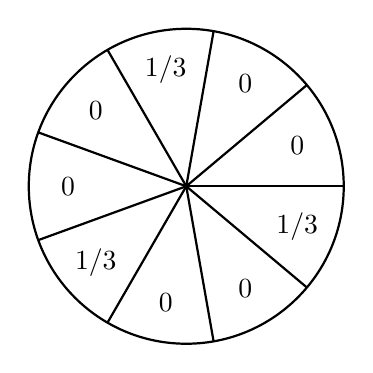
\begin{tikzpicture}
\def\radius{2.cm}
\def\txtradius{1.5cm}

% cercle extérieur
\draw[thick] (0,0) circle (\radius);

% tracer les rayons pour 9 parts
\foreach \i in {0,...,8} {
  \draw[thick] (0,0) -- (\i*40:\radius); % 360/9 = 40
}

% labels écrits à la main
\node at (20:\txtradius) {0};
\node at (60:\txtradius) {0};
\node at (100:\txtradius) {1/3};
\node at (140:\txtradius) {0};
\node at (180:\txtradius) {0};
\node at (220:\txtradius) {1/3};
\node at (260:\txtradius) {0};
\node at (300:\txtradius) {0};
\node at (340:\txtradius) {1/3};
\end{tikzpicture}
\end{center}
Supposons qu’Alice commence par prendre une part de poids $0$. Alors Bob mange immédiatement le $1/3$ adjacent. En continuant à suivre la stratégie consistant à prendre systématiquement la part révélée par Alice, Bob finit (après avoir concédé un $1/3$ à Alice) par obtenir un deuxième $1/3$.  
Inversement, si Alice commence par une part de poids $1/3$, alors Bob peut s’assurer de manger les deux autres $1/3$ en suivant la règle suivante : 
\begin{itemize}
    \item si un $1/3$ est disponible, Bob le prend ; 
    \item si un $0$ voisin d’un $1/3$ est disponible, Bob choisit l’autre.
\end{itemize}

\item Voici le code Python utilisé pour déterminer la pizza de Bob. 
Comme le dénominateur du ratio dans la question vaut $9$, on peut raisonnablement supposer que le poids total de la pizza à trouver (avant normalisation) est de $9$. 
Dans le code ci-dessous, la recherche est donc restreinte aux pizzas dont le poids total est $9$, avec des parts entières. 
On utilise un algorithme de programmation dynamique. Sur un ordinateur portable classique, l'exécution de l'algorithme prend environ 50 secondes à trouver une solution. Enfin, on remarque qu'une démonstration (sans recours au calcul informatique) est possible, mais elle suppose de connaître préalablement la solution afin de pouvoir l'analyser.

\begin{lstlisting}
(*@\codeheader{\currfiledir/4.py}@*)
(*@ @*)
\end{lstlisting}
\vspace{-.455cm}
\lstinputlisting{\currfiledir/4.py}

La pizza solution est la suivante :

\begin{center}
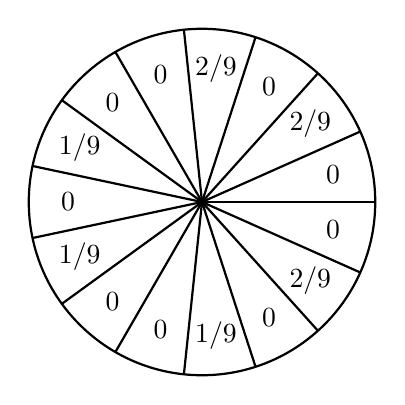
\begin{tikzpicture}
\def\radius{2.2cm}

% cercle extérieur
\draw[thick] (0,0) circle (\radius);

% tracer les rayons pour 9 parts
\foreach \i in {0,...,14} {
  \draw[thick] (0,0) -- (\i*24:\radius); % 360/9 = 40
}

% labels écrits à la main
\node at (12:1.7) {0};
\node at (36:1.7) {2/9};
\node at (60:1.7) {0};
\node at (84:1.7) {2/9};
\node at (108:1.7) {0};
\node at (132:1.7) {0};
\node at (156:1.7) {1/9};
\node at (180:1.7) {0};
\node at (204:1.7) {1/9};
\node at (228:1.7) {0};
\node at (252:1.7) {0};
\node at (276:1.7) {1/9};
\node at (300:1.7) {0};
\node at (324:1.7) {2/9};
\node at (348:1.7) {0};
\end{tikzpicture}
\end{center}


\item On regarde le cas $n$ impair et on reprend les notations de la question~\ref{Montrez qu’Alice peut manger au moins le tiers de la pizza en suivant une stratégie où}.

\begin{definition}[Propriété des verts lourds]
\leavevmode
\begin{itemize}
    \item  $[C_1, C_2]_0$ a la propriété des verts lourds si, pour tout $[C_1, C]_0 \subseteq [C_1, C_2]_0$, on a 
    \(
        |V([C_1, C]_{0})| \ge |R([C_1, C]_{0})|.
    \)
    \item  $[C_1, C_2]_{1}$ a la propriété des verts lourds si, pour tous $[C_1, C]_0, [C_2, C']_0 \subseteq [C_1, C_2]_1$, on a 
    \(
        |V([C_2, C']_{0})| \ge |R([C_2, C']_{0})|\) et \(
               |V([C_1, C]_{0})| \ge |R([C_1, C]_{0})|.
    \)
\end{itemize}
\end{definition}

\begin{definition}[Meilleure réponse de Bob] 
Lorsque Alice joue la stratégie suivre-Bob après qu'un intervalle impair $[C_1, C_2]_1$ soit déjà mangé, le comportement de Bob revient à choisir une coupe $C$ séparant $[C_1, C_2]_0$ en deux intervalles pairs $[C, C_1]_0$ et $[C, C_2]_0$.  
Dans ce cas, Alice obtient
\(
R([C, C_1]_0) \cup R([C, C_2]_0),
\)
et Bob obtient
\(
V([C, C_1]_0) \cup V([C, C_2]_0).
\)
On appelle meilleure réponse de Bob à $[C_1, C_2]_1$ toute coupe $C$ qui minimise la quantité
\(
\big| R([C, C_1]_0) \cup R([C, C_2]_0) \big|,
\)
parmi toutes les coupes $C$ telles que $[C, C_1]_0 \subseteq [C_1, C_2]_0$. Si $[C_1, C_2]_1$ ne contient qu'une seule part, 
on dit que $C$ est une meilleure réponse à une part unique (mrpu).  
Dans ce cas, la stratégie sB d'Alice est dite associée à $C$.
\end{definition}

\begin{lemma}[des verts lourds]
Soit $C$ telle que $[C, C_1]_0 \subseteq [C_1, C_2]_0$. Alors $C$ est une meilleure réponse à $[C_1, C_2]_1$ si et seulement si $[C, C_1]_0$ et $[C, C_2]_0$ possèdent la propriété des verts lourds.
\end{lemma}

\begin{proof}
Une coupe $C$ est une meilleure réponse à $[C_1, C_2]_1$ si et seulement si pour toute coupe $\widetilde{C}$ avec $[C, \widetilde{C}]_0 \subseteq [C_1, C_2]_0$, on a
\(
|R([C, C_1]_0) \cup R([C, C_2]_0)| \le |R([ \widetilde{C},C_1]_0) \cup R([\widetilde{C},C_2]_0)|.
\)
Comme
\begin{align*}
R([C, \widetilde{C}]_0) \subseteq R([C, C_1]_0) \cup R([C, C_2]_0), \quad
V([C, \widetilde{C}]_0) \subseteq R([ \widetilde{C},C_1]_0) \cup R([\widetilde{C},C_2]_0),
\\
 (R([C, C_1]_0) \cup R([C, C_2]_0))\backslash R([C, \widetilde{C}]_0) = 
  (R([ \widetilde{C},C_1]_0) \cup R([\widetilde{C},C_2]_0))\backslash V([C, \widetilde{C}]_0),
\end{align*}
on a que
l’inégalité précédente est équivalente à
\(
|V([C, \widetilde{C}]_0)| \ge |R([C, \widetilde{C}]_0)|,
\)
ce qui correspond à la propriété des verts lourds pour $[C, C_1]_0$ si $[C, \widetilde{C}]_0 \subseteq [C, C_1]_0$ et pour $[C, C_2]_0$ sinon.
\end{proof}

\begin{definition}[Pizza facile et pizza dure]
On dit qu’une pizza est facile si Alice dispose d’une stratégie sB lui garantissant au moins la moitié de la pizza.  
Sinon, la pizza est dite dure.
\end{definition}

\begin{lemma}[des pizzas faciles]
Si deux coupes voisines $C$ et $C'$ sont chacune une mrpu, alors la pizza est facile.
\end{lemma}
\begin{proof}
Alice peut garantir
\(
\max\bigl( \vert R([C, C]_{1})\vert, \, \vert R([C', C']_{1})\vert \bigr)
\)
en choisissant la meilleure des deux stratégies sB associées à $C$ et $C'$.
Soit $p$ la part comprise entre $C$ et $C'$.  
Comme 
\(
R([C', C']_{1}) \;=\; V([C, C]_{1}) \cup \{p\},
\) 
on en déduit que 
\(
R([C, C]_{1}) \cup R([C', C']_{1})
\)
recouvre toute la pizza.
 En particulier, l'un des deux recouvre la moitié de la pizza.
\end{proof}

\begin{theorem}[des pizzas dures]
Si une pizza est dure et que  
\(
C_1 \in \arg\min_{C} \, |R([C, C]_{1})|,
\)
alors il existe deux mrpu $C_2$ et $C_3$ qui partitionnent la pizza en trois intervalles impairs disjoints
\(
[C_1, C_2]_{1},  [C_1, C_3]_{1}, [C_2, C_3]_{1},
\)
chacun possédant la propriété des verts lourds.
\end{theorem}

\begin{proof}
    Pour une coupe $C$, on note $A(C)$ l’ensemble des parts uniques dont $C$ est une meilleure réponse.
    \begin{itemize}
    \item On choisit $C_2 \in \arg\max_{\text{mrpu}~C}|R([C, C]_{1})|$ de façon à maximiser $|A(C_2) \setminus A(C_1)|$.
    \item On choisit $C_3$ comme une meilleure réponse à la part $\hat{p} \in V([C_1,C_2]_{1})$ la plus proche de $C_2$.
\end{itemize}
Les colorations canoniques de $[C_1,C_1]_{1}$ et $[C_2,C_2]_{1}$ coïncident sur $[C_1,C_2]_{1}$ et sont inversées sur $[C_2,C_1]_{0}$. Ainsi, si $C_2$ est une meilleure réponse à une part $p \in [C_1,C_2]_{1}$, alors $C_1$ l’est également. Autrement dit :
\begin{equation*} 
A(C_2) \setminus A(C_1) \subseteq R([C_2, C_1]_{0}).
\end{equation*}
Soit $\widetilde{p}$ la dernière part de $A(C_2) \setminus A(C_1)$ en parcourant $[C_2,C_1]_{0}$ depuis $C_2$.  
Les parts $\hat{p}$ et $\widetilde{p}$, avec la coupe $C_2$, divisent la pizza en trois intervalles, dont un se réduit à une seule part.

\textbf{Affirmation.} La coupe $C_3$ se situe dans l’intervalle entre $C_2$ et $\widetilde{p}$ ne contenant pas $\hat{p}$.
\begin{proof}[Preuve de l’affirmation]
Si $C_3$ est dans l’intervalle entre $\hat{p}$ et $C_2$ ne contenant pas~$\widetilde{p}$, 
alors $C_3$ et $C_2$ sont voisines, et la pizza est facile par le lemme des pizzas faciles, contradiction.

Supposons maintenant que $C_3$ soit dans l’intervalle entre $\hat{p}$ et $\widetilde{p}$ ne contenant pas $C_2$.  
Comme $C_3$ est une meilleure réponse à $\hat{p}$, on a $\hat{p} \in [C_3,C_2]_{0}$ (car $\hat{p}\in V([C_2,C_2]_1)$), donc $\widetilde{p}\in [C_3,C_2]_{1}$ et on a 
\[
A(C_2) \setminus A(C_1) \subseteq R([C_3,C_2]_{1}) \subseteq R([C_3,C_3]_{1}).
\]
Cela signifie que $C_3$ est une réponse possible de Bob à toutes les parts de $A(C_2)\setminus A(C_1)$.  
Comme $C_2$ est une meilleure réponse à toutes les parts de $A(C_2)\setminus A(C_1)$, on a
\(
|R([C_2,C_2]_{1})| \leq |R([C_3,C_3]_{1})|.
\)
Mais comme $C_3$ est aussi une mrpu, et que $C_2$ maximise $|R([C_2,C_2]_{1})|$ sur les mrpu, on a égalité, et $C_3$ est une meilleure réponse à toutes les parts de $A(C_2)\setminus A(C_1)$
et aussi à $\hat{p} \notin A(C_2)\setminus A(C_1)$, contredisant la règle de choix de $C_2$.
\end{proof}
D’après l’affirmation, $C_3$ est situé dans $[C_2,C_1]_{0}$. Comme $\hat{p} \in R([C_3,C_3]_{1})$, la coupe $C_3$ sépare $[C_1,C_2]_{0}$ en deux intervalles impairs, donnant une partition en trois intervalles impairs
\[
[C_1,C_2]_{1}, \quad [C_1,C_3]_{1}, \quad [C_2,C_3]_{1}.
\]
On considère à présent la coloration cannonique des chacun de ces intervalles. On a que chaque $C_i$ est une meilleure réponse à une part verte dans l'intervalle opposé:
\begin{itemize}
    \item $C_1$ est une meilleure réponse à toutes les parts de $R([C_1,C_1]_1)\supseteq V([C_2,C_3]_1)\neq \emptyset$ car sinon la pizza est facile par le lemme des pizzas faciles, 
    \item $C_2$ est une meilleure réponse à $\widetilde p \in V([C_1,C_3]_1)$,
    \item $C_3$ est une meilleure réponse à $\hat{p}\in V([C_1,C_2]_1)$.
\end{itemize}
Par le lemme des verts lourds,  
chacun des intervalles vérifie la propriété des verts lourds. 
Pour chaque intervalle, on applique le lemme deux fois : une fois avec chacune de ses extrémités, 
celles-ci jouant le rôle de la coupe $C$, tandis que la part verte située dans l’intervalle opposé à $C$ 
joue le rôle de l’intervalle impair dans le lemme.  
On obtient ainsi successivement les deux conditions nécessaires, ce qui établit la propriété des verts lourds 
pour l’intervalle impair considéré.
\end{proof}

\begin{notation}[pizza partielle]
On considère l’intervalle impair $[C_2, C_3]_{1}$ comme une pizza indépendante, obtenue en supprimant les deux autres intervalles et en recollant les coupes $C_2$ et $C_3$.  
La pizza ainsi obtenue est appelée pizza partielle et la coupe issue du recollement est notée $C_{2,3}$.
Comme $[C_2, C_3]_{1}$ vérifie la propriété des verts lourds, la coupe recollée $C_{2,3}$ de la pizza partielle appartient à $\arg\min_{C} |R([C, C]_{1})|$ ($\arg\min$ sur les coupes de la pizza partielle).
\end{notation}


\begin{notation}
Pour $i \in \{1,2,3\}$, on note $R_i$ l’ensemble des parts rouges de l’intervalle impair 
opposé à $C_i$, et $r_i$ leur poids total, par exemple 
$r_2 = |R_2| = |R([C_1, C_3]_1)|$.  
De même, on note $V_i$ l’ensemble des parts vertes de l’intervalle impair opposé à $C_i$, 
et $v_i$ leur poids total, par exemple 
$v_1 = |V_1| = |V([C_2, C_3]_1)|$.  
Supposons qu’Alice joue une stratégie sB associée à une coupe $C \in \{C_1, C_2, C_3\}$.
Alors Alice obtient au moins $|R([C, C]_1)|$, ce qui peut s’exprimer en fonction des $r_i$ et $v_i$ comme dans le tableau suivant :  

\[
\begin{array}{|c|c|c|}
\hline
\text{Coupe} & \text{Gain d’Alice} & \text{Gain de Bob} \\
\hline
C_1 & v_1 + r_2 + r_3 & r_1 + v_2 + v_3 \\
C_2 & r_1 + v_2 + r_3 & v_1 + r_2 + v_3 \\
C_3 & r_1 + r_2 + v_3 & v_1 + v_2 + r_3 \\
\hline
\end{array}
\]
Par définition de $C_1$ (resp. $C_2$), le gain $v_1 + r_2 + r_3$ (resp. $r_1 + v_2 + r_3$) 
est le plus petit (resp. le plus grand) des trois gains possibles pour Alice. 
On a donc
\[
v_1 + r_2 + r_3 \;\le\; r_1 + r_2 + v_3 \;\le\; r_1 + v_2 + r_3.
\]
D'autre part, puisque la pizza est dure, chacun des gains d’Alice dans le tableau est 
strictement inférieur à $\tfrac{1}{2}$, et donc strictement inférieur au gain de Bob. 
En sommant chaque paire d’inégalités ainsi obtenues, on en déduit que, pour tout 
$i \in \{1,2,3\}$, on a $v_i > r_i$. 
On note $p_i \in V_i$ la part "centrale" telle que la somme des poids de toutes les parts vertes à partir de $p_i$ (incluse) dans chaque direction jusqu’à rencontrer une coupe dans $\{C_1, C_2, C_3\}$ est au moins égale à $\frac{v_i}{2}$.
\end{notation}

\begin{definition}[Stratégie sB modifiée, sBm]
Pour $i \in \{1,2,3\}$, la $i$-ième stratégie sBm, notée $\text{sBm}_i$, est définie comme suit~:  
\begin{enumerate}
    \item Alice commence en mangeant $p_i \in V_i$.
    \item Tant que les coups de Bob révèlent des pièces dans $V_i$, Alice les prend également, c’est-à-dire qu’elle suit Bob.
    \item Au moment où le coup de Bob révèle la première pièce rouge d’un autre des trois intervalles impairs, Alice effectue un seul coup où elle ne suit pas Bob, en prenant une pièce dans $R_i$.
    \item Alice suit Bob à partir de ce moment jusqu’à la fin du jeu.
\end{enumerate}
Ainsi, une stratégie sBm contient exactement un coup d’Alice où elle ne suit pas Bob. Après ce coup particulier, un intervalle impair $[C, C_j]_1 \subseteq [C_i, C_j]_1$ avec $C_i \neq C_j \in \{C_1, C_2, C_3\}$ est entièrement mangé. Alice suit alors Bob après que cet intervalle soit mangé.
D’après le lemme suivant, soit $C_i$ soit $C_j$ est une meilleure réponse à tout intervalle impair $[C, C_j]_1 \subseteq [C_i, C_j]_1$.  
Dans le pire des cas, Alice obtient donc soit $r_i + v_j$, soit $v_i + r_j$ en dehors de $[C_i, C_j]_1$.  
La plus petite de ces deux quantités peut donc être considérée comme le gain garanti d’Alice.  
En combinant cela avec la définition de la pièce centrale $p_i$, on obtient donc les gains garantis suivants pour les stratégies sBm :

\[\begin{array}{|c|c|}
\hline
\text{Stratégie sBm} & \text{Gain garanti pour Alice} \\
\hline
\text{sBm}_1 & \frac{v_1}{2} + v_2 + r_3 \\
\text{sBm}_2 & v_1 + \frac{v_2}{2} + r_3 \\
\text{sBm}_3 & v_1 + r_2 + \frac{v_3}{2}
\\
\hline
\end{array}\]
\end{definition}


\begin{lemma}[des sBm]
Pour une pizza dure, soient $C_i, C_j\in \{C_1, C_2, C_3\}$ deux coupes distinctes et $C$ telle que
\([C, C_j]_1 \subseteq [C_i, C_j]_1\). Alors $C_i$ ou $C_j$ est une meilleure réponse 
à $[C, C_j]_1$.
\end{lemma}

\begin{proof}
Supposons qu’il existe une coupe $\widetilde{C} \notin \{C_i, C_j\}$ qui soit une meilleure réponse 
à $[C, C_j]_1$. Comme on a 
\([\widetilde C, {C}_j]_0 \subseteq [C, C_j]_0\), on obtient aussi 
\([\widetilde C, {C}_i]_0 \subseteq [C, C_j]_0\).  
Ainsi, soit \([\widetilde C, {C}_i]_0\), soit \([\widetilde C, {C}_j]_0\) est entièrement contenu 
dans un des trois intervalles de la tripartition.
D’après le Théorème des pizzas dures, chaque intervalle de la tripartition vérifie la propriété des verts lourds. 
On en déduit que, pour $k = i$ ou $k = j$, on a \(
|V([C_k, \widetilde{C}]_0)| \ge |R([C_k, \widetilde{C}]_0)|.
\)
Comme $\widetilde{C}$ est une meilleure réponse, le lemme des verts lourds implique
\(
|V([\widetilde C, {C}_k]_0)| \ge |R([\widetilde C, {C}_k]_0)|,
\)
i.e.,
\(
|V([C_k, \widetilde{C}]_0)| = |R([C_k, \widetilde{C}]_0)|.
\)
Ainsi,
\(
|R([\widetilde C, {C}]_0) \cup R([\widetilde C, {C}_j]_0)| 
= |R([C_k, C]_0) \cup R([C_k, C_j]_0)|.
\)

Cela montre que $C_k \in \{C_i, C_j\}$ est aussi une meilleure réponse à $[C, C_j]_1$. 
\end{proof}

\begin{lemma}[de la pizza partielle]
Considérons une pizza avec un nombre impair de parts (pas nécessairement dure), 
et un état intermédiaire du jeu dans lequel l’intervalle pair $[C,C']_{0}$ est mangé, 
où $C \in \arg\min_C |R([C, C]_{1})|$.  
Soient $p$ et $p'$ les parts adjacentes à $C$ et $C'$, respectivement, mais non comprises 
dans $[C,C']_{0}$. Alors, si Alice choisit $p'$ et suit ensuite Bob, elle obtient au moins autant que si elle choisit $p$ et joue ensuite de façon optimale.\end{lemma}

\begin{proof}
Supposons qu’Alice choisisse $p'$ puis suive Bob. $C \in \arg\min_C |R([C, C]_{1})|$, donc l’intervalle impair $[C,C]_{1}$ vérifie la propriété des verts lourds.  
Par le lemme des verts lourds, $C$ est alors une meilleure réponse à l’intervalle $[C,C']_{0} \cup \{p'\}$.  
Ainsi, dans le pire des cas, Alice obtient les parts rouges $R([C,C']_{1})$ et Bob les parts vertes $V([C,C']_{1})$.
D’un autre côté, si Alice choisit $p$ et joue ensuite au mieux, Bob peut forcer la même distribution 
en suivant simplement Alice jusqu’à ce que toute la pizza soit mangée.  
Par conséquent, choisir $p'$ et suivre Bob ne peut jamais donner un résultat moins bon.
\end{proof}

\begin{definition}[Stratégie bonne pour la pizza partielle]
 On dit qu’une stratégie pour la pizza partielle est bonne si, au moment où $C_{2,3}$ est révélé, 
  elle prescrit déjà à Alice de suivre Bob (dans la pizza partielle) jusqu’à la fin du jeu (bien entendu, dans le contexte 
de la pizza entière, Alice ne peut pas appliquer directement cette instruction).
   Une stratégie bonne est dite connectée à la pizza entière si les conditions suivantes sont vérifiées :
  \begin{enumerate}
    \item Alice commence dans $[C_2,C_3]_{1}$ comme s’il s’agissait de la pizza partielle, et y applique la stratégie bonne tant que ni $C_2$ ni $C_3$ ne sont révélées.
    \item Si Bob révèle $C_2$ ou $C_3$ (ce qui correspond à $C_{2,3}$ dans la pizza partielle), 
    alors Alice joue selon la première variante du lemme de la pizza partielle plutôt que la seconde.
    \item Chaque fois que Bob choisit une part en dehors de $[C_2,C_3]_{1}$, Alice suit Bob.
  \end{enumerate}
\end{definition}

\begin{lemma}
Une bonne stratégie connectée à la pizza entière garantit à Alice au moins le gain garanti par cette stratégie dans la pizza partielle, plus $r_2 + v_3$.
\end{lemma}

\begin{proof}
Puisque la stratégie dans la pizza partielle est bonne, le lemme de la pizza partielle assure qu’à l’intérieur de $[C_2,C_3]_{1}$, Alice obtient au moins le gain garanti par cette stratégie pour la pizza partielle.
En effet, tant que la coupe $C_{2,3}$ n’est pas révélée, la partie se déroule uniquement 
dans la pizza partielle et Alice suit alors sa stratégie. Lorsque $C_{2,3}$ 
est finalement révélée, elle applique la première variante du lemme, ce qui lui garantit 
un résultat au moins aussi bon que celui qu’elle aurait obtenu dans avec sa stratégie
dans la pizza partielle.
À l’extérieur de $[C_2,C_3]_{1}$,  Alice suit Bob après qu’un intervalle impair $[C,C_2]_{1} \subseteq [C_2,C_3]_{1}$ ou $[C,C_3]_{1} \subseteq [C_2,C_3]_{1}$ a été mangé. Or, d’après le lemme des sBm, une meilleure réponse est alors donnée soit par $C_2$, soit par $C_3$.  
Ainsi, dans le pire des cas, Alice obtient soit $r_2 + v_3$, soit $v_2 + r_3$ en dehors de $[C_2,C_3]_{1}$.  
Or, on a $r_2 + v_3 \leq v_2 + r_3$.   
\end{proof}

\begin{theorem}Alice peut manger au moins $4/9$ de n'importe quelle pizza.
\end{theorem}

\begin{proof}
Considérons d'abord la pizza partielle et distinguons deux cas.

\textbf{Cas 1. La pizza partielle est facile.} \\
Par définition, il existe une stratégie sB pour la pizza partielle assurant à Alice au moins la moitié de son poids. Chaque stratégie sB est une bonne stratégie et peut donc être connectée à la pizza entière. Considérons trois stratégies d'Alice pour la pizza entière :  
\begin{enumerate}
    \item La stratégie sB associée à $C_2$, qui garantit au moins $r_1 + v_2 + r_3$,
    \item La stratégie sBm, notée $\text{sBm}_2$, qui garantit au moins $v_1 + \frac{v_2}{2} + r_3$,
    \item La stratégie sB connectée à la pizza entière, qui garantit au moins $\frac{v_1+r_1}{2} + r_2 + v_3$ (par le lemme précédent).
\end{enumerate}
Le ratio de $\frac{4}{9}$ se démontre en calculant une moyenne appropriée de ces stratégies (au moins l'une de ces trois stratégies assure donc à Alice un gain moyen de $\frac{4}{9}$) :
\begin{align*}
&\frac{3}{9}(r_1+v_2+r_3) + \frac{2}{9}\left(v_1+\frac{v_2}{2}+r_3\right) + \frac{4}{9}\left(\frac{v_1+r_1}{2}+r_2+v_3\right) \geq \frac{4}{9}(r_1+v_1+r_2+v_2+r_3+v_3). 
\end{align*}
\textbf{Cas 2. La pizza partielle est dure.} \\
D'après le Théorème des pizzas dures, la pizza partielle peut être tripartitionnée par la coupe $C'_1 \triangleq C_{2,3}$ et deux autres meilleures réponses $C'_2$ et $C'_3$ en trois intervalles impairs disjoints possédant la propriété des verts lourds.  
On utilise la notation abrégée habituelle pour les poids totaux des parts rouges et vertes dans ces intervalles, par exemple $r'_1 = |R([C'_2,C'_3]_1)|$ et $v'_2 = |V([C'_1,C'_3]_1)|$.
La stratégie sB pour la pizza partielle associée à $C'_2$, ainsi que la stratégie $\text{sBm}_1$ pour la pizza partielle, sont des bonnes stratégies et peuvent être connectées à la pizza entière. Nous considérons quatre stratégies d'Alice pour la pizza entière :  
\begin{enumerate}
    \item La stratégie sB associée à $C_2$, donnant au moins $r_1 + v_2 + r_3$,
    \item La stratégie $\text{sBm}_2$, donnant au moins $v_1 + \frac{v_2}{2} + r_3$,
    \item La stratégie sB associée à $C'_2$ connectée à la pizza entière, donnant au moins $r'_1 + v'_2 + r'_3 + r_2 + v_3$ (lemme précédent),
    \item La stratégie $\text{sBm}_1$ connectée à la pizza entière, donnant au moins $\frac{v'_1}{2} + v'_2 + r'_3 + r_2 + v_3$ (lemme précédent).
\end{enumerate}
On a donc
\begin{align*}
&\frac{3}{9}(r_1 + v_2 + r_3) 
+ \frac{2}{9}\left(v_1 + \tfrac{v_2}{2} + r_3\right) 
+ \frac{2}{9}\left(r'_1 + v'_2 + r'_3 + r_2 + v_3\right) 
+ \frac{2}{9}\left(\tfrac{v'_1}{2} + v'_2 + r'_3 + r_2 + v_3\right)\\&\geq
\frac{3}{9}(v_2+r_3+r_1) + \frac{2}{9}(\tfrac{v_2}{2}+r_3+v_1) + \frac{2}{9}(r_2+v_3+v_1) + \frac{2}{9}(r_2+v_3+\tfrac{r_1}{2})
\\&\ge \frac{4}{9}(r_1+v_1+r_2+v_2+r_3+v_3).
\end{align*}
en utilisant
$v'_2+r'_3\ge r'_2+v'_3$
et $r_1 = v'_1 + r'_2 + r'_3$ et $v_1 = r'_1 + v'_2 + v'_3$.
\end{proof}


\end{enumerate}


\subsection*{Notes et références}

Le \emph{problème de la pizza de Winkler} a été posé par Peter Winkler lors de la conférence 
\emph{Building Bridges}, en l'honneur du 60\ieme{} anniversaire de László Lovász, à Budapest en 2008.  
La borne optimale connue de $\tfrac{4}{9}$ a été obtenue indépendamment dans deux travaux : \cite{cibulka2009solution} et \cite{knauer2011eat}. La présente solution est basée sur ce dernier travail.
Un problème voisin a été étudié dans un contexte plus général :  
deux joueurs se partagent un graphe connexe dont les sommets portent des poids non négatifs.  
À tour de rôle, ils choisissent un sommet et collectent son poids, en respectant la règle que la partie restante du graphe doit rester connexe après chaque coup.  
Ce jeu est connu sous le nom de \emph{graph-grabbing game}, étudié par \cite{micek2011graph}.


\bibliography{\currfiledir/sources.bib}
\newpage